
\def\layersep{2.5cm}

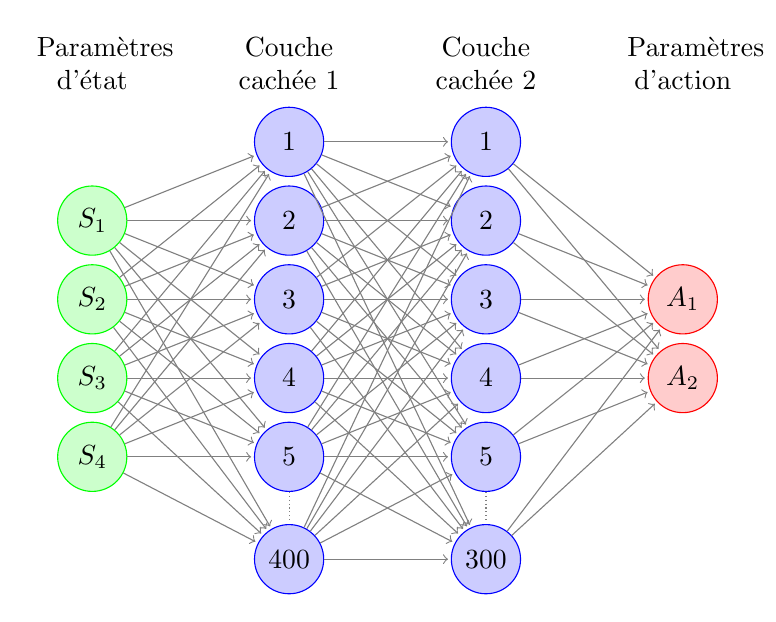
\begin{tikzpicture}[shorten >=1pt,->,draw=black!50, node distance=\layersep, scale = 1]
    \tikzstyle{every pin edge}=[<-,shorten <=1pt]
    \tikzstyle{neuron}=[circle,fill=black!25,minimum size=25pt,inner sep=0pt]
    \tikzstyle{input neuron}=[neuron, fill=green!20, draw=green];
    \tikzstyle{output neuron}=[neuron, fill=red!20, draw=red];
    \tikzstyle{hidden neuron}=[neuron, fill=blue!20, draw=blue];
    \tikzstyle{annot} = [text width=4em, text centered]

    % Draw the input layer nodes
    \foreach \name / \y in {1,...,4}
    % This is the same as writing \foreach \name / \y in {1/1,2/2,3/3,4/4}
        \node[input neuron] (I-\name) at (0,-1-\y) {$S_{\name}$};


    % Draw the hidden layer nodes
    % H1
    \foreach \name / \y in {1,...,5}
        \node[hidden neuron] (H1-\name) at (\layersep,-\y) {$\name$};
    \path[yshift=-0.3cm]
    		node[hidden neuron] (H1-6) at (\layersep,-6) {$400$};
    		
    	% H2
    \foreach \name / \y in {1,...,5}
        \node[hidden neuron] (H2-\name) at (2*\layersep,-\y) {$\name$};
    \path[yshift=-0.3cm]
    		node[hidden neuron] (H2-6) at (2*\layersep,-6) {$300$};

    		

    % Draw the output layer node
    \foreach \name / \y in {1,...,2}
     	\node[output neuron] (O-\name) at (3*\layersep,-2-\y) {$A_{\name}$};


	% ...
	\foreach \ID in {H1,H2}
		\path (\ID-5) edge[-,densely dotted] (\ID-6);

	
	% Connect layers
	\foreach \source in {1,...,4}
	{
        \foreach \dest in {1,...,6}
        {
        		% input layer to first hidden layer
        		\path (I-\source) edge (H1-\dest); 
		}
			  	
	}
	\foreach \source in {1,...,6}
	{
		\foreach \dest in {1,...,6}
        {
			% hidden layers
			\path (H1-\source) edge (H2-\dest);
		}
		\foreach \dest in {1,...,2}{
			% hidden layer 2 to output
            \path (H2-\source) edge (O-\dest);
		}
	}
            

    % Annotate the layers
    \node[annot,above of=H1-1, node distance=1cm] (h1) {Couche cachée $1$};
    \node[annot,above of=H2-1, node distance=1cm] (h2) {Couche cachée $2$};
    \node[annot,left of=h1] {Paramètres d'état};
    \node[annot,right of=h2] {Paramètres d'action};
\end{tikzpicture}